\documentclass[12pt]{article}
\usepackage[a4paper, left=2cm, right=2cm, top=2cm]{geometry}
\usepackage[natbibapa]{apacite}
\usepackage[hyphens,spaces]{url} \usepackage[colorlinks,citecolor=blue,urlcolor=blue]{hyperref}
\usepackage{hyperref}% http://ctan.org/pkg/hyperref
\hypersetup{%
	colorlinks = true,
	linkcolor  = black
}
\usepackage[english]{babel}
\usepackage[T1]{fontenc}
\usepackage[onehalfspacing]{setspace}
\usepackage[autostyle]{csquotes}
\usepackage{graphicx}


\usepackage{multirow,booktabs,setspace,caption}
\usepackage{tikz}

\usepackage{amsmath}

% apa table
\DeclareCaptionLabelSeparator*{spaced}{\\[2ex]}
\captionsetup[table]{textfont=it,format=plain,justification=justified,
	singlelinecheck=false,labelsep=spaced,skip=0pt}
\captionsetup[figure]{labelsep=period,labelfont=it,justification=justified,
	singlelinecheck=false,font=doublespacing} 

% equations 
\usepackage{bm}
\usepackage{bbm}

% tables 
\usepackage{wrapfig,lipsum,booktabs}

% plot
\usepackage{graphicx}
\usepackage{subcaption}

\begin{document}
	
\title{Glacier Movement Prediction with Deep Learning Models and Satellite Data}
\author{Jonas Müller}
\maketitle

\begin{abstract}

\end{abstract}


\tableofcontents
\section{Introduction}
Glaciers and their inherent dynamics are a well documented indicator for global climate change impact \citep{abram2019framing, zemp2008global, avian2020status,dyurgerov2000twentieth, stoffel2012effects,shrestha2015integrated, mazhar2021effects, scambos2017much, yu2023bibliometric, berthier2023measuring}. While in addition 10 \% of the Earth’s land area is covered by glaciers or ice sheets, which in total hold about 69\% of Earth’s freshwater \citep{gleick1996water}, it is of crucial importance to study and monitor glacial changes over time. In adition to global sea level changes due to cryospheric changes, glacier melting can have local impacts on close regions like landslides, debris flows, rock slope failures, or ice avalanches \citep{stoffel2012effects}. In order to study the impacts of glacial change advanced remote sensing approaches have been developed cosisting of e.g. terrestial laserscanning, radar satellite applications, unmanned aerial vehicels, automatic camera imaging and \textit{multispectral satellite imaging} \citep{avian2020status}. In multispectral satellite imaging the spectral reflectance of glacier surfaces is captured by sensors on the satllite. These sensors are sensitive to different bands in the light reflectance spectrum and are then used to estimate the composition of the underlying terrain, e.g. snow, ice, rocks or water \citep{kaab2014glacier}. From the green ($0,53-0,59 \mu m $, resolution: 30 m) and the shortwave infrared band ($1.57-1.65 \mu m$, resolution 30m) the \textit{Normalized Snow Difference Index} [NDSI] can be calculated for example as a measure indicating snow/ice covered land masses.

\begin{figure}[h]%[htp]
	
	\centering
	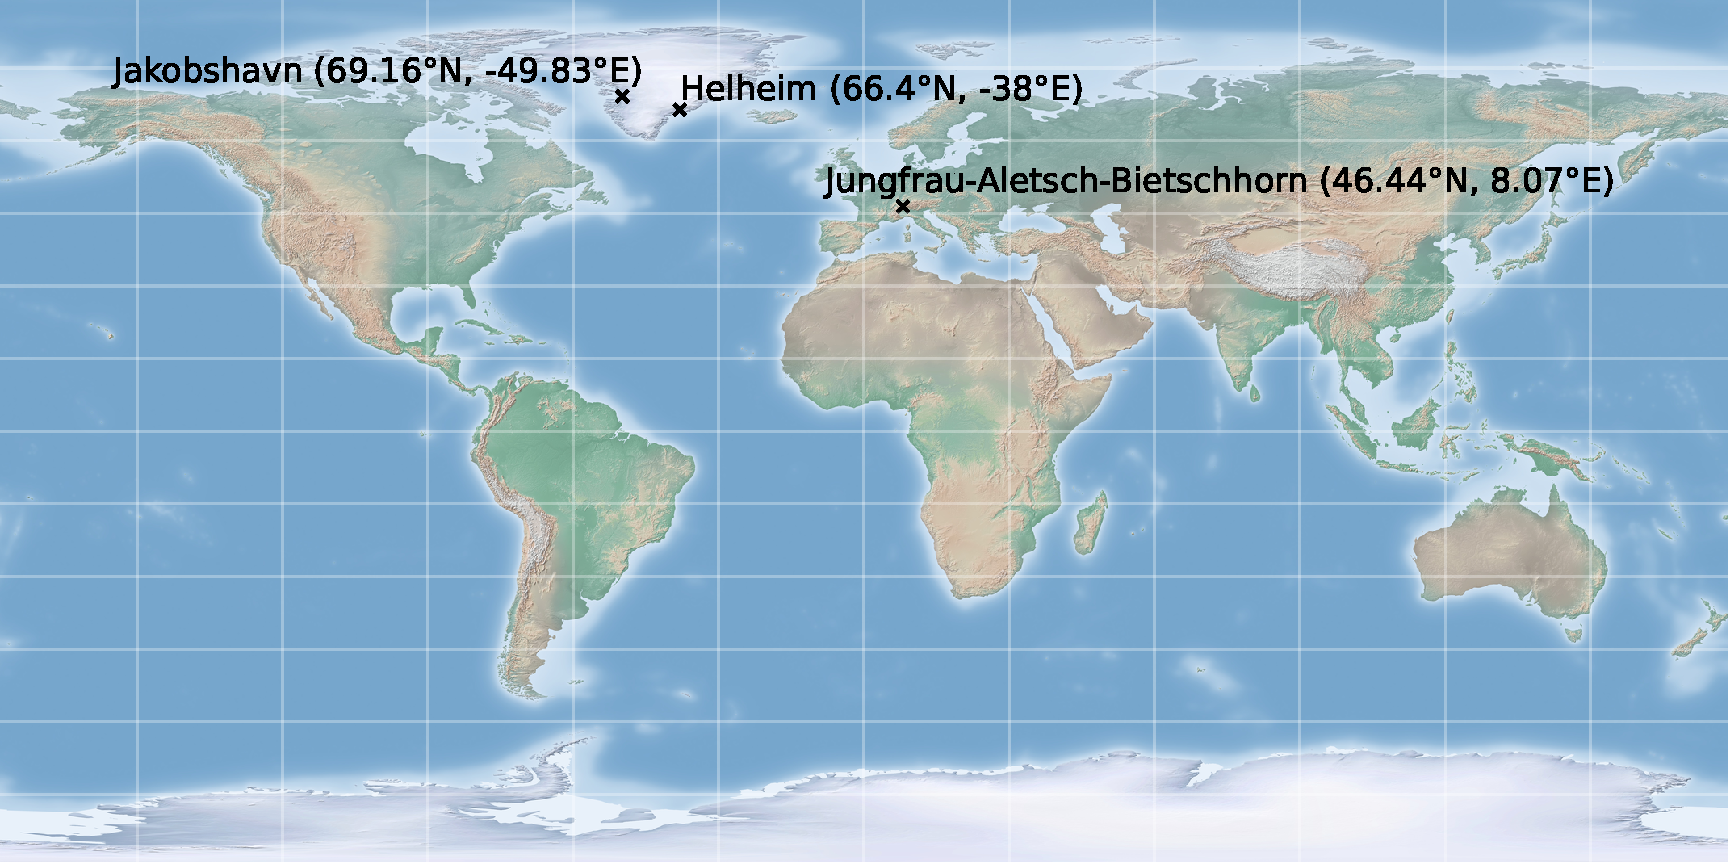
\includegraphics[scale = 0.581]{map.pdf}
	\newline
	\newline
	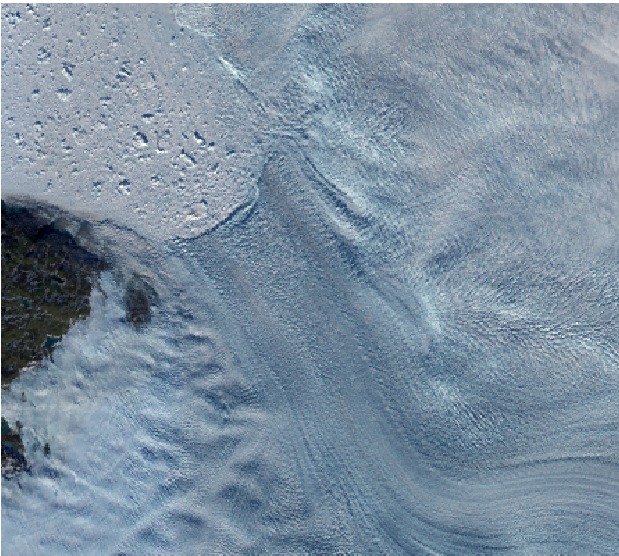
\includegraphics[width=.3\textwidth]{jakobshavn.pdf}\hfill
	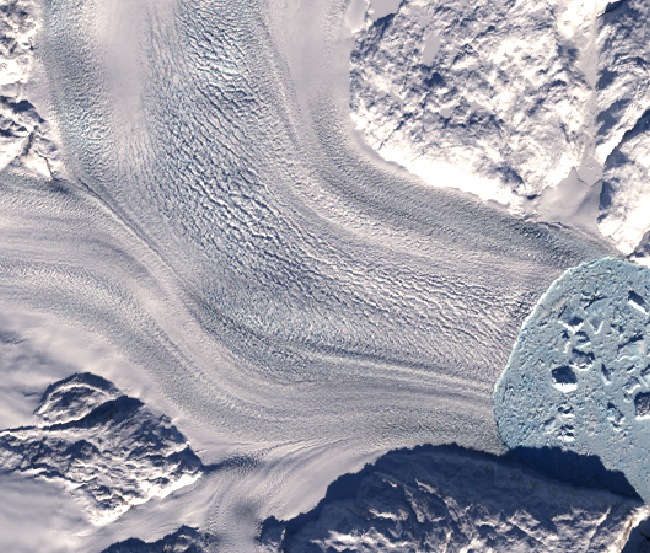
\includegraphics[width=.3\textwidth]{helheim.pdf}\hfill
	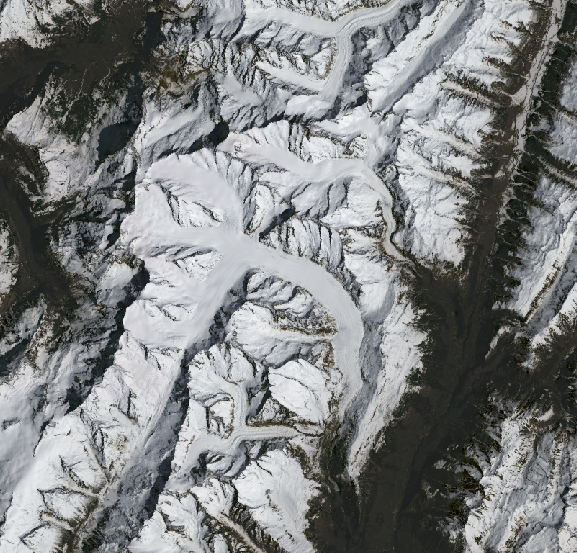
\includegraphics[width=.3\textwidth]{aletsch.pdf}
	
	
	\caption{Overview of the studied glaciers. The Images are extracted from Landsat-8 spectral bands and plotted in RGB coordinates.}
	\label{fig:figure1}
	
\end{figure}

Many models of glacier dynamics explicitly focus on the physical processes inside glaciers \citep{colgan2016glacier, berthier2023measuring}. This aproach comes with the disadvantage of varying estimates of diffferent models, varying uncertainties of different data sources, varying estimates of the same models by different research groups and the need of required explicit knowledge of the underlying processes for parameter estimation and data prediction. Therefore deep learning methods have been deployed for glacier movement prediction from satellite data \citep{min2019predicting}, where glacier dynamics are modeled indirectly through input-output relations. Due to the ability to learn complex recurrent patterns and the emergence and improvement of advanced neural network architectures in the theoretical deep learning literature, e.g. long short-term memory networks \citep{hochreiter1997long}, convolutional autoencoders \citep{DBLP:journals/corr/RonnebergerFB15} or transformer models \citep{vaswani2017attention}, the use of higher computational resources in model training \citep{anthony2020carbontracker} and larger datasets, the deep learning research domain has made large progresses, especially in the field of computer vision \citep{chai2021deep}. Based on these promising findings the present study therefore focuses on the application of recurrent deep learning models to time series satellite image data of different glaciers. For this task landsat-8 satellite image data (figure \ref{fig:figure1}), is used, with which deep learning models are trained and tested. The used models are adapted from the theoretical literature in computer vision deep learning research, representing state of the art approaches in image processing.

\subsection{Related Work}

While many studies are focused on satellite image classification with machine learning approaches [e.g. \citet{chu2022glacier, marochovautomated, prieur2022machine}], few studies are exploring the prediction of future glacier states with recurrent neural networks [RNN]. Many studies on the other hand focus on the prediction of sea ice motion with RNN [e.g. \citet{mu2023icetft, zhai2021machine, petrou2017prediction, petrou2019prediction}]

\citet{min2019predicting} for example are stressing the importance of machine learning applications in the realm of climate science problems. In their study the authors developed a method to predict ice flow movements of the byrd glacier in antarctica with satellite data from the landsat-8 imaging system. The authors used correlations of image patches in a given scene to patches from another scene to find a matching target patch as ground truth for ice movement, thus tracking ice flow in a dynamic region of interest between scenes. The authors used 2 long term-short term memory [LSTM] layers in order predict scene patches with stochastic video generation, thereby conditioning a prior network on previous subscenes. 

\citet{petrou2017prediction} used a LSTM encoder-decoder architecture \citep{srivastava2015unsupervised} in order to predict future patches of artic sea ice motion satellite imaging scenes. They used the Advanced Microwave Scanning Radiometer - Earth Observing System [AMSR-E] from NASA's aqua satellite in order to calculate optical flow patches for each pair of consecutive days. The authors improved this network by using convolutional LSTM cells, which switches multiplication operations in the LSTM cell with convolution operations and works on the images directly instead of vector representations \citep{petrou2019prediction} 

\citet{ali2021sea} used an attention based ensemble LSTM approach in order to predict sea ice motion from a mix of ERA-5 global reanalysis product data and Nimbus-7 satellite data. The authors then used both monthly and daily data in two sepearte LSTM layer branches, where each branch has an attention mechanism that calculates attention weights for the different hidden states, therefore evading the bottleneck problem of accumulating context information in LSTM models in the hidden state representation and instead using full self attention in order to not loose any important context information.   

\citet{mu2023icetft} furthermore developed a LSTM-transformer hybrid model, the \textit{ice temporal fusion transformer} for sea ice motion prediction. The network in addition uses physical variables like cloud-microphysics, thermodynamics or radiation as input to the network in order to predict sea ice changes over time. Up to this timepoint no research papers are known that use transformer neural networks for glacier movement prediction from satellite image data. Therefore this paper presents an unique opportunity to provide a contribution in the understanding of a large climate change detection indicator. 

\section{Methodology}
\subsection{Dataset}
The generated dataset consists of landsat-8 level 2 satellite images of multiple glaciers. For the acquisition of the image data the SpatioTemporal Asset Catalog [STAC] was used. The catalog can be accessesd with an API using Microsofts Planetary Computer, a cloud consisting of environment data for scientific investigations. The satellite images (\textit{Scenes}) were filtered for cloud coverage and amount of missing values. Scenes were excluded if they had more than 20 \% of cloud coverage and more than 50 \% of missing pixel values. The scenes come with 19 bands consisting of 11 different spectral bands with a spatial resolution of $30m$ per pixel, measuring light reflectance spectra, and different bands supplying additional information, e.g. a band giving spatial information of cloud coverage for pixels. From the spectral bands 2 bands were used to estimate glacier movements: the green band ($0,53-0,59 \mu m $, resolution: 30 m) and the shortwave infrared band ($1.57-1.65 \mu m$, resolution 30m). These bands are used to create the NDSI. This index quntifies a continuous measure of snow/ice. In addition \citet{he2020glacier} already used the NDSI in order to classify glaciers with a U-net architecture. In order to further quantify snow/ice in pixels a threshold of 0.3 is used \citep{vonica2021glacier}. With this threshold masks are generated, indicating snow, where the value for each pixel is generated as:
	$$
	 p_{i,z} = \left\{
	\begin{array}{ll}
		NDSI(p_{i,z}) & NDSI(p_{i,z}) \geq 0.3 \\
		0 & \, else,  \\
	\end{array}
	\right. $$
	

	
 In order to capture each glacier fully, large regions are used, e.g. 800x800 pixels for the parvati glacier. Because of that, the scenes are sampled in patches of size (50, 50) to decrease the computational load of the used models. In order to generate the final model input, patches of the same coordinates in different scenes are used over time, therefore sampling the same region at different timepoints. The models get 4 patches from different consecutive scenes as an input
 $\{a_{k, t} \in A, b_{k, t+1} \in B, c_{k, t+2} \in C, d_{k, t+3} \in D, \;  k \in K,  t \in T\}$ and predict the next 4 patches in the same coordinates $\{f_{k, t+4} \in F, g_{k, t+5} \in G, h_{k, t+6} \in H, i_{k, t+7} \in I,\;  k \in K,  t \in T \}$, where $k$ denotes the patch number and $t$ the time index.  Because the intervals between scenes are not evenly spaced (e.g. exclusions because of clouds or missing data) the scenes are averaged over months (3 months in 1. experiment, 6 months in second experiment). Thus the model input and target dimensions, ignoring the batch dimension, in summary are 4x50x50 tensors.
 
 The different bands of the satellite contain some amount of missing pixel values which is why a kernel is used to average out missing values. The procedure is adapted from \citet{vonica2021glacier}. The Kernel selects missing pixels, places a 5x5 kernel on top of the missing value, replaces all missing pixels in the respective image space the kernel is targeted at with 0, and calculates a weighted average for the missing pixel in question.
 
 Because landsat-8 imaging is not completely accurate \citep{vonica2021glacier}, an allignment procedure is used to compensate for pixel shifts in images to produce more robust model predictions. For this the enhanced correlation coefficient maximization algorithm is used \citep{evangelidis2008parametric}. The algorithm iteratively refines an estimate of alignment paramters, e.g. image translation transformations by maximiziing the \textit{enhanced correlation coefficient} between two images. First a mean image is created with all images of the scene and then all scenes are aligned to this mean image with translation transformations on parallel lines. This transformation moves the scenes without rotating and scaling, is therefore computationally fast, should leave no bias in the scenes (e.g. aligning pixels that actually represent glacier movements) and improves the prediction accuracy of the models. 
 
Glacier movements are characterized by seasonal and annual changes \citet{sam2018heterogeneity}. Figure \ref{fig:figure3} shows the estimated optical flow between two consecutive scenes from the parvati glacier with a 3 month timedelta. For the optical flow estimation the dense optical flow algorithm by \citet{farneback2003two} is used. In comparison to sparse optical flow algorithms which use only a small subset of pixels for motion estimation, dense optical flow algorithms estimate the movement of every pixel in the image. The algorithm uses a image pyramid which smoothes and resamples the image at multiple levels (resampling factor: 0.5, levels of pyramid: 6, thus decreasing the size of the image by a factor of 0.5). At each level of the pyramid the algorithm uses quadratic polynomials in order to estimate the local local brightness changes between the two images. The algorithm uses 10 iterations at each level of the pyramid. All other parameters are adapted to their standard values \citep{vonica2021glacier}. Figure \ref{fig:figure3} shows two aligned consecutive scenes of the parvati glacier and estimated optical flow vectors. In order not to populate the whole scene with motion vectors the vectors are only drawn every 40 pixels (1200 meter).
 
 %The algorithm uses \textit{ORB} features, a mixture of the fast accelerated segment test [FAST] keypoint detector and binary robust independent elementary features [BRIEF] in order to find matching keypoints between two images. The images are then aligned based on feature matches using the random sample consensus [RANSAC] algorithm \citep{derpanis2010overview}.  
	
	
%	\begin{figure}[htp]
		
	%	\centering
	%	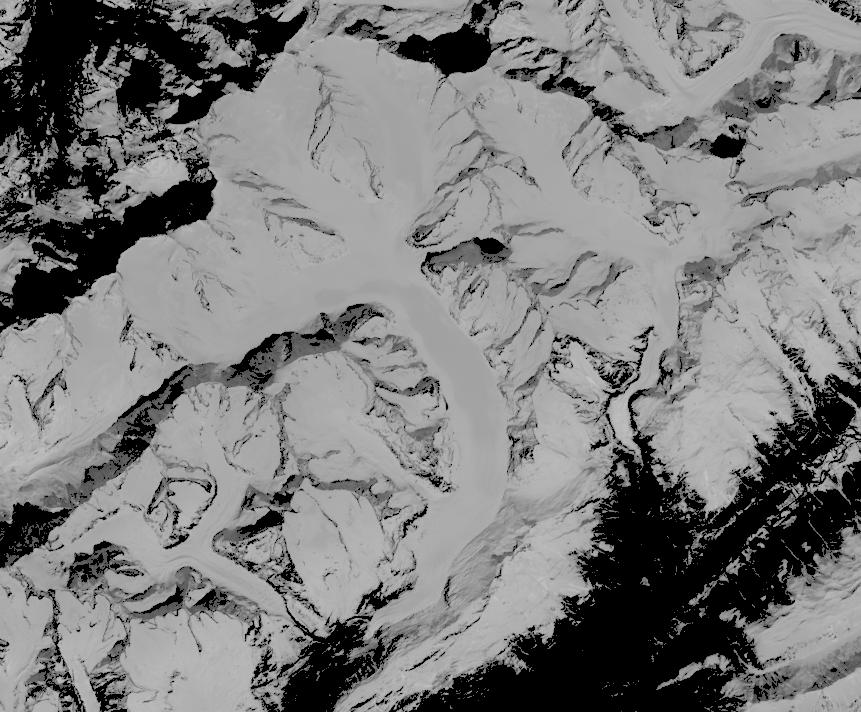
\includegraphics[scale = 0.5]{aletschSnow.jpg}\hfill
		
	%	\caption{Snow mask extracted from the generated NDSI index map. Scene taken from  Jungfrau-Aletsch-Bietschhorn Glacier ($46.477 ^{\circ} N, 8.056^{\circ} E$) on the 23 of March 2015.}
	%	\label{fig:figure2}
		
	%\end{figure} 
\begin{figure}[h]
	
	\centering
	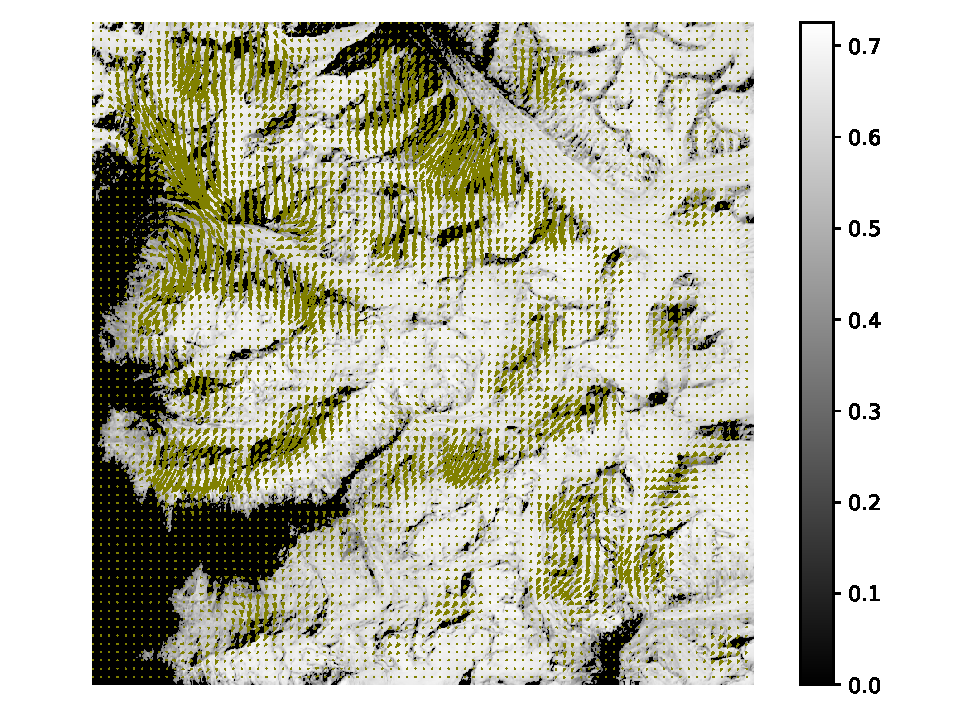
\includegraphics[scale = 0.25]{parbatiFlow.pdf}\hfill
	
	\caption{Dense optical flow estimated from two consecutive scenes with $\Delta_t = 3$ months (left: average over April, Mai and June 2013; right: Juli, August and September 2013) of the parvati glacier.}
	\label{fig:figure3}
	
\end{figure} 

\subsection{Models}
While some of the used models are adapted from the theoretical literature and are inspired by previous work on sea-ice motion prediction (e.g. \citet{petrou2019prediction, petrou2017prediction}), therefore using LSTM and convolutional LSTM cells, other models are used because of their successes in other vision tasks, e.g. the U-net architecture \citep{ronneberger2015u} in biomedical image segmentation. Interestingly \citet{holzmann2021glacier} used an U-net with an attention mechanism for glacier calving front segmentation, showing the applicability of U-net to satellite glacier data. The third class of used models consists of transformer models. These are selected because of their recent success in language processing, image classification and video prediction \citep{khan2022transformers}. In addition transformer models have the added benefit of no vanishing gradient problem, no fuzzy context accumulation problems because of information accumulation, e.g. in LSTM cells, and the capacity to generalize to arbitrary long sequences by design of the architecture \citep{vaswani2017attention}. 

As described above, all models get 4 consecutive scene patches as input and predict the next 4 consecutive patches in the same coordinates. The models are trained with the mean squared error loss function [MSE] over all predicted future patches resulting in:

\begin{equation}
	MSE = \frac{\sum_{i}^{N} \sum_{t}^{T} \sum_{x}^{X} \sum_{y}^{Y} (\tilde{y}_{i, t, x, y} - y_{i, t, x, y})^2}{N \times T \times X \times Y },
\end{equation}
where $\tilde{y}$ represents the snow mask prediction of the model at timepoint and $y$ represents the snow mask ground truth. In addition $i\in N$ represents the index of the training example, $t \in T$ the time index, $x \in X$ the image width coordinate and $y \in Y $ the image height coordinate.  

\subsubsection{LSTM model}
The first model uses the LSTM cell developed by \citet{hochreiter1997long}. The LSTM cell has four different gates that are used recursively in order to predict sequential data (equation \ref{lstm}). The LSTM cell gets a hidden state representation, a cell state representation and a flattened input patch vector as an input. The central idea is that context information is accumulated and integrated at each timestep in the hidden and cell states. In the beginning the hidden and cell states are initialized as tensors containing 0 values. The different gate activations are then calculated with the following equations (note that vectors and matrices are bold):  


\begin{equation}
	\begin{aligned}
		\mathbf{i} &= \sigma(\mathbf{W}_{ii}\mathbf{x} + \mathbf{b}_{ii} + \mathbf{W}_{hi}\mathbf{h} + \mathbf{b}_{hi}), \\
		\mathbf{f} &= \sigma(\mathbf{W}_{if}\mathbf{x} + \mathbf{b}_{if} + \mathbf{W}_{hf}\mathbf{h} + \mathbf{b}_{hf}), \\
		\mathbf{g} &= \mathrm{tanh}(\mathbf{W}_{ig}\mathbf{x} + \mathbf{b}_{ig} + \mathbf{W}_{hg}\mathbf{h} + \mathbf{b}_{hg}), \\
		\mathbf{o} &= \sigma(\mathbf{W}_{io}\mathbf{x} + \mathbf{b}_{io} + \mathbf{W}_{ho}\mathbf{h} + \mathbf{b}_{ho}), \\
		\mathbf{c'} &= \mathbf{f} \odot \mathbf{c} + \mathbf{i} \odot \mathbf{g}, \\
		\mathbf{h'} &= \mathbf{o} \odot \mathrm{tanh}(\mathbf{c'}),
	\end{aligned}
	\label{lstm}
\end{equation}

where $\mathbf{W}$ consitutute weight matrices, $\mathbf{b}$ additive biases, $\mathbf{h}$ hidden state representations, $tanh$ the tangent hyperbolic activation function, $\sigma$ the sigmoid activation function, $\mathbf{c^{\prime}}$ the new cell state, $\mathbf{h^{\prime}}$ the updated hidden state, $\mathbf{x}$ the new incoming input and $\odot$ signifies the Hadamard product. The indices of the weight matrices and bias vectors represent firstly, if the weight matrix is multiplied by the input or the hidden state, and secondly, to which gate the matrix belongs to. In addition the different gates are connected through \textit{peephole connections} \citep{gers2002learning}, therefore allowing information flow between gates in each cell state update. 

The differnt gates were explicitly designed for different functionalities.  The forget gate ($\mathbf{f}$) controls how much of the previous hidden state is remembered by integrating the last hidden state with the input $\mathbf{x}$ by outputting values between 0  and 1 on a continuous scale qunatifying remembering (towards 1) and forgetting (towards 0). The input gate ($\mathbf{i}$) integrates the input with the last hidden state in order to quantify how much of the new information is integrated into the cell state. The output gate ($\mathbf{o}$) quantifies how much of the calculated cell state is integrated in the new hidden state (which is also the output of the LSTM cell for each timestep). The candidate gate ($\mathbf{g}$) quantifies how much of the input gate is added to the cell state.

In the optimization process the backpropagation algorithm is then used across timesteps, thus gradients are accumulated across timesteps backwards through time, so called \textit{backpropagation through time}. The LSTM cell does not suffer from vanishing gradients by design as the gating mechanism in the forget gate controls the gradient flow in the internal recurrence of the cell. This can be seen in the derivative of the cell state: 

\begin{equation}
	\frac{\partial \mathbf{c'}}{\partial \mathbf{c}} \mathbf{f} \odot \mathbf{c} + \mathbf{i} \odot \mathbf{g} = \mathbf{f},
\end{equation}

as the derivative of the cell state with respect to itself is always a vector of 1 (the so called \textit{constant error carousel} \citep{hochreiter1997long}). If the biases in the forget gate are initialized with high values, the gradients never vanish or explode as both bounds are regulated by the forget gate, which learns its activation across training. 

The used model is an encoder decoder architecture with LSTM cells, which uses the input in the encoder, copys cell and hidden states to the decoder and then recurrently predicts into the future by using the model predictions from previous timesteps.

\subsubsection{Convolutional LSTM Network}
The next model has a similar structure to the LSTM network described above, with the difference, that now instead of vector representations of image patches, the patches itself are fed into the network. Therefore all the matrix multiplication operations now become convolution operations: 

\begin{equation}
	\begin{aligned}
		\mathbf{i} &= \sigma(\mathbf{W}_{ii} * \mathbf{x} + \mathbf{W}{hi} * \mathbf{h} + \mathbf{b}_{hi}), \\
		\mathbf{f} &= \sigma(\mathbf{W}_{if} * \mathbf{x} + \mathbf{W}_{hf} * \mathbf{h} + \mathbf{b}_{hf}), \\
		\mathbf{g} &= \mathrm{tanh}(\mathbf{W}_{ig} * \mathbf{x} + \mathbf{W}_{hg} * \mathbf{h} + \mathbf{b}_{hg}), \\
		\mathbf{o} &= \sigma(\mathbf{W}_{io} * \mathbf{x} + \mathbf{W}_{ho} * \mathbf{h} + \mathbf{b}_{ho}), \\
		\mathbf{c'} &= \mathbf{f} \odot \mathbf{c} + \mathbf{i} \odot \mathbf{g}, \\
		\mathbf{h'} &= \mathbf{o} \odot \mathrm{tanh}(\mathbf{c'}),
	\end{aligned}
	\label{conv_lstm}
\end{equation}

The used network also uses a encoder-decoder structure with a recurrent future prediction module.

\subsubsection{Convolutional U-net Autoencoder}
The network structure of the U-net follows a contracting and an expanding path in a fully convolutional architecture with 23 layers \citep{ronneberger2015u}. The main idea of the network is to increase the channel dimensions in the contracting path in such a way that information of the image is abstracted into a large number of feature maps, while descending into the latent space with decreasing image size. The used skip connections project intermediate feature maps from the same part of the contracting to the expanding path horizontally, therefore protect the network from information loss over long distances in the network and increase stability of predictions.

The contracting path uses a typical convolutional network architecture consisting of repeated 3x3 convolutions, ReLU activations, and 2x2 max pooling operations with downsampling. At each downsampling step, the number of feature channels is doubled. In the expansive path the feature maps are upsampled followed by a 2x2 convolution that halves the number of feature maps again, then the cropped feature map (necessary due to the loss of border pixels in every convolution) from the corresponding part of the contracting path is concatenated and two 3x3 convolutions are performed, which are followed by ReLu activation functions. The final layer consists of a 1x1 convolutional layer in order to map the channel dimension back to 1 for prediction. 

\subsubsection{Self Attention Transformer Model}
\begin{equation}
\begin{aligned}
	\text{Attention}(Q, K, V) &= \text{softmax}\left(\frac{QK^T}{\sqrt{d_k}}\right)V \
\end{aligned}
\end{equation}

\citet{vaswani2017attention}

\subsubsection{Vision Transformer Model}




\section{Experiment 1: Prediction of Patches}
\subsection{Parvati Glacier}
The Parvati glacier is well suited for the prediction of glacier movmements, because first the landsat-8 image catalog provides a high temporal density of scenes that are almost evenly distributed over the months in a year, and second because of the high glacier density in the region and the surroundings. Therefore a dataset was created in which scenes are averaged over the months of each year from January 01, 2013 until January 01, 2021. If for a given month no scenes were available the missing months were interpolated linearly in order to prevent temporal bias in the data. The patches were extraced from the provided coordinates (\ref{fig:figure1}) in regions of interest of 800x800 pixels with a stride of 10, resulting in 566048 sequences of 4 scenes and 4 corresponding targets. the data was then splitted into 80\% training and 20\% test data, while 10\% of the training data was used for validation. The dataset was firstly used in order to test the different model architectures and get an understanding of the best performing architectures. In order to curtail the the architecture and parameter space a set of models was tested. This set contained two transformer models \citep{vaswani2017attention}, two vision transformer models adapted to predict sequences of patches over time  \citep{dosovitskiy2020image}, a LSTM encoder-decoder model with future prediction module \citep{srivastava2015unsupervised}, and a U-net model adapted to predict patches over time recurrently \citep{ronneberger2015u}. As data augmentation techniques teacher forcing, dropout, weight decay and early stopping were used 



\begin{center}
	\begin{tabular}{|c|c|c|}
		\hline
		Model & MSE & MAE \\
		\hline
		Unet & 0.0658 & 0.1810 \\
		\hline
		Transformer & 0.0668 & 0.2268 \\
		\hline
		LSTM & 0.0545 & 0.1651 \\
		\hline
		Vision Transformer & 0.0843 & 0.2085 \\
		\label{key} \\
		\hline
	\end{tabular}
\end{center}


\section{Experiment 2: Fine Tuning on Different Glaciers}

\section{Experiment 3: Gneralisation to Full Scenes}
\subsection{Full Scene Learning}
 In a next step the models are retrained and fine-tuned in order to predict full scenes across time. In order to achieve this the models should learn smooth borders between patches of each scene in order to create a full consistent image. Thus a new dataset is used containing only non overlapping patches from consecutive scenes. 
 
 Two approchaes are tested to achieve this. In the first approach the model now takes a sequence of scenes, e.g. $\{A, B, C, D, E\}$ and predicts the next $n$ patches for the next scenes, e.g. $\{F, G, H, I, J, ...\}$ in the future. Therefore the model input is now $\{a_k \in A, b_k \in B, c_k \in C, d_k \in D, e_k \in E\} \ \forall k \in K$, where $K$ is the number of respective patches in each scene, while the model output is now $\{f_k \in F, g_k \in G, h_k \in H, i_k \in I, j_k \in J\} \ \forall k \in K$ (all patches with the same indices stem from the same coordinates in the scene). After the model predicted all patches for the next secenes they are put together again from the patches and a final MSE loss is calculated on the full scenes and propagated through the model. With this procedure the model then learns to smooth the edges of the patches in the full scene image.
\subsection{U-net Denoising Autoencoder}
 
 

\subsection{Results}
\subsection{Generalisation Test}

\section{Discussion}
carbon footprint of model training
dimensionality reduction techniques for image vector embeddings
\section{Limitations}

\section{Summary}





\newpage

% Bibliiography¸
\bibliographystyle{apacite}
\bibliography{references}

\end{document}